\subsection{Schnittstellenbeschreibungen}
Das folgende Kontextdiagramm (Abbildung \ref{fig:kontextdiagramm}) zeigt eine Übersicht über das System und sämtlichen Schnittstellen. In den folgenden Abschnitten werden die Schnittstellen im Detail beschrieben.

\begin{figure}[h!]
	\centering
	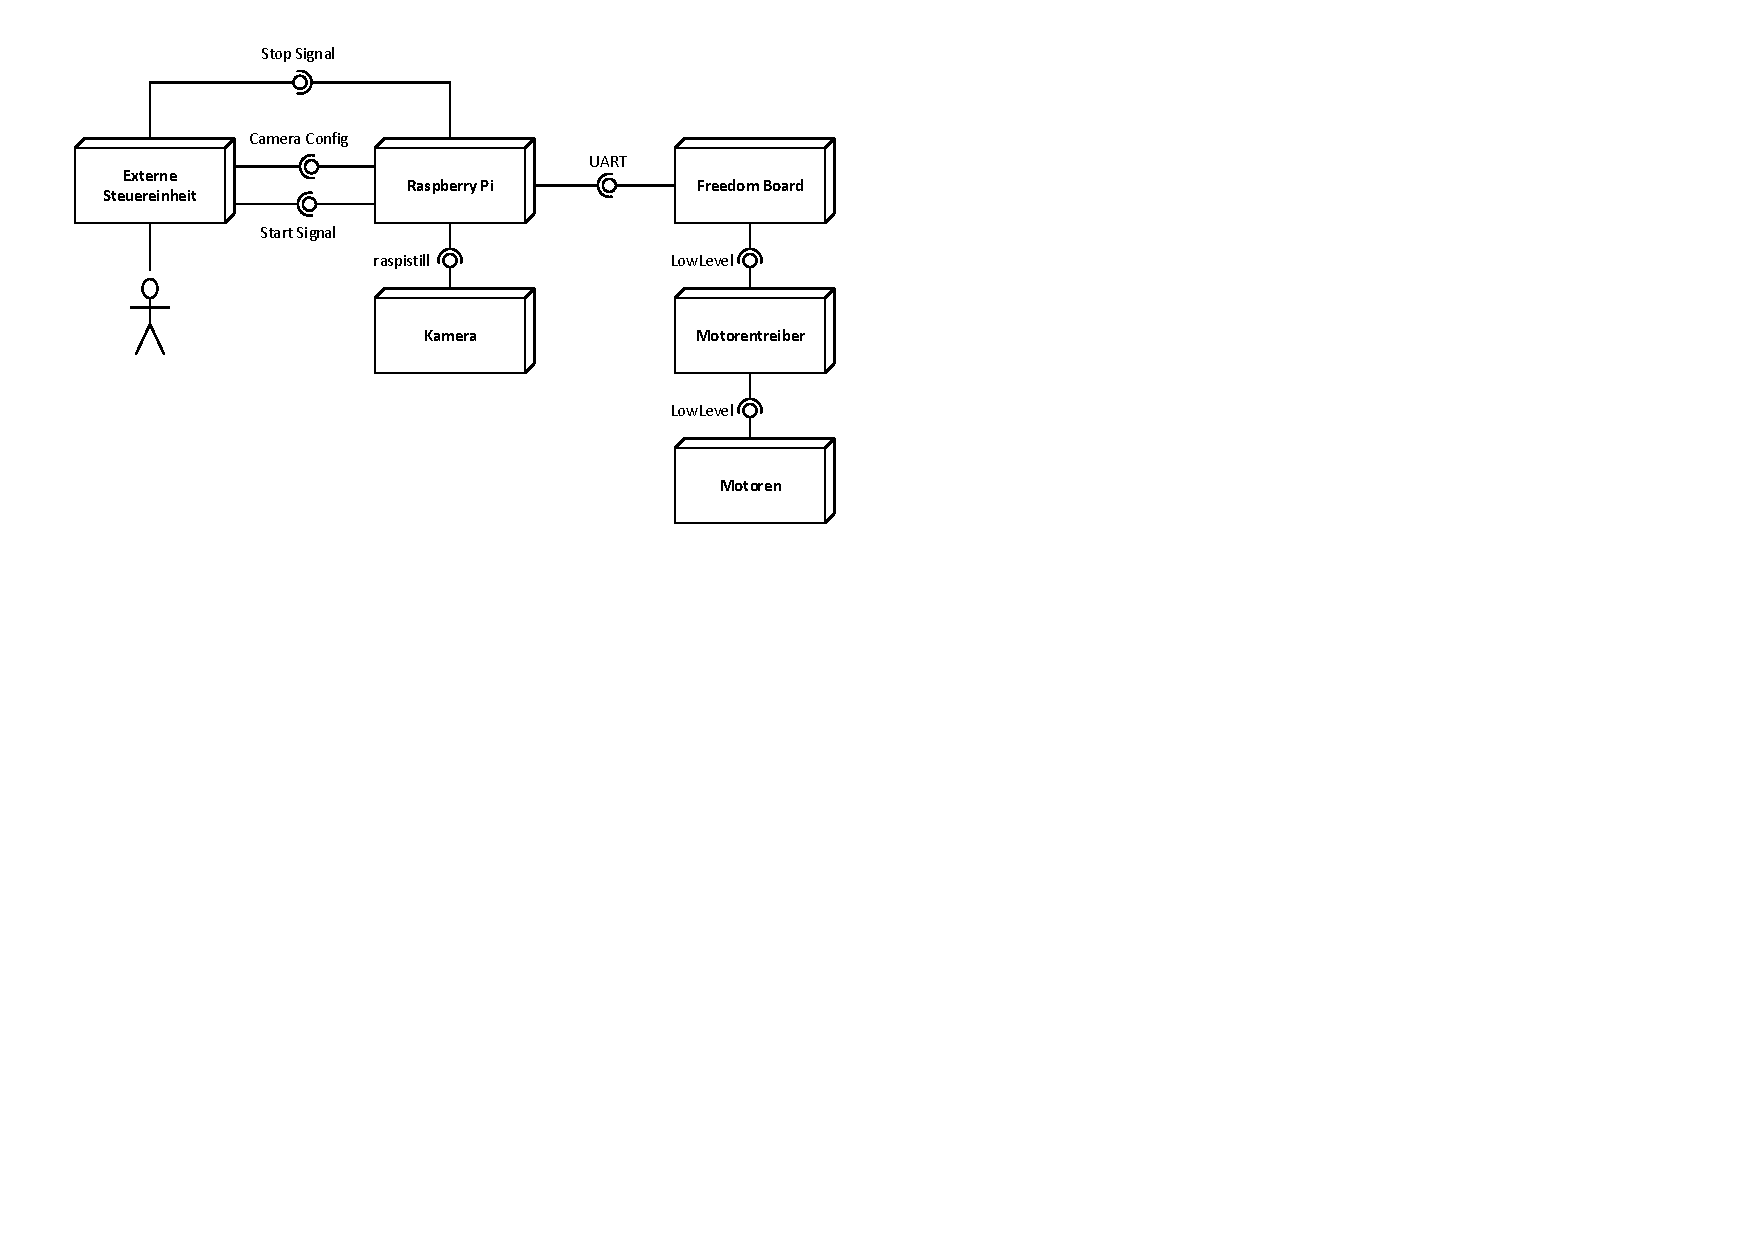
\includegraphics[width=0.9\linewidth]{../../fig/kontextdiagramm}
	\caption{Kontextdiagramm}
	\label{fig:kontextdiagramm}
\end{figure}

Die Schnittstellen Start Signal, Stop Signal und Camera Config werden von einem Webserver als REST\footnote{Representational State Transfer}-Ressourcen zur Verfügung gestellt. Dadurch wird der Aufrufer nicht auf eine bestimmte Programmiersprache beschränkt. Zudem können die Schnittstellen in der Testphase mit einem einfachen Browser angesteuert werden.

TODO REST-Schnittstelle des Start Signals beschreiben

\subsubsection{Stop Signal}
Die Schnittstelle Stop Signal wird vom Webserver auf der externen Steuereinheit angeboten. Die Adresse von diesem Webserver ist dem Raspberry Pi, durch das Start Signal, bekannt. Wenn das Programm auf dem Raspberry Pi beendet ist, schickt es einen PUT-Request an den Webserver auf der externen Steuereinheit und signalisiert so das Stop Signal. Tabelle \ref{tab:put-stop-signal} zeigt ein Beispiel der Anfrage.

\begin{table}[h!]
	\centering
	\begin{tabular}{|l|l|}
		\hline Anfrage an externe Steuereinheit	 & Antwort von externer Steuereinheit \\ 
		\hline \verb|PUT /stop-signal HTTP/1.1|  & \verb|200 OK| 					  \\
			   \verb|Host: 192.168.1.3| 		 & 							          \\
		\hline 
	\end{tabular} 
	\caption{PUT-Request an Stop Signal}
	\label{tab:put-stop-signal}
\end{table}

Durch dieses Design muss die externe Steuereinheit nicht permanent nach dem Status des Programms fragen (Polling). Der Webserver auf der externen Steuereinheit verarbeitet den Request und gibt das Stop Signal visuell aus.

\newpage

TODO REST-Schnittstelle der Camera Config beschreiben

\newpage

TODO raspistill beschreiben und Verweiss auf Doku im Internet \href{http://www.raspberrypi.org/wp-content/uploads/2013/07/RaspiCam-Documentation.pdf}{Link zu Doku}

Die UART Schnittstelle dient der Kommunikation zwischen Raspberry Pi und
dem Freedomboard, welches die LowLevel Funktionalität der Maschine 
umsetzt. Dieses implementiert sämtliche Ansteuerng von Hardwarekomponenten
wie Motorentreibern oder Sensoren. Die übergeordnete Instanz des Freedomboards
ist das Raspberry Pi, welches die Schnittstelle zum Benutzer bildet. Die für
diese Abstraktion notwendige Schnittstelle wird mittels UART
implementiert. Ein mögliches Protokoll ist in der Tabelle \ref{tab:uart}
zusammengefasst.

Die serielle Schnittstelle wird vom Freedomboard direkt implementiert auf
USB mittels einer USB-Seriell Wandlung. Dies ermöglicht es, das Freedomboard
direkt per USB-Kabel am Raspberry Pi zu verbinden.

\begin{table}[h!]
	\centering
	\begin{tabular}{l l l l l}
		Aktion & Message & Parameter & Antwort \\
		\hline
		drehen um $\varphi$ 
			& \verb!rotate!
			& Winkel $\varphi$
			& aktuelle Position \\
		Entfernung $s$ setzen
			& \verb!distance!
			& Entfernung $s$
			& aktuelle Entfernung \\
		Ausrichtungsmotor enable
			& \verb!rotater!
			& enable/disable
			& aktueller status\\
		Schussmotor enable
			& \verb!shooter! 
			& enable/disable
			& aktueller Status \\
		Lademotor enable
			& \verb!loader!
			& enable/disable
			& aktueller status\\
		Schussabgabe
			& \verb!fire!
			& -
			& ok/nok\\
		Reset
			& \verb!reset!
			& -
			& -\\
	\end{tabular}
	\caption{Protokollentwurf der seriellen Schnittstelle}
	\label{tab:uart}
\end{table}


\subsubsection{LowLevel}
Als LowLevel Schnittstellen werden die einfachen Ansteuerungen
bezeichnet, welche direkt mittels eines Mikrocontroller erzeugt
werden.

Die einzelnen Hardwarekomponenten wie Motorentreiber werden mittels
einfachen digitalen Signalen bedient. Dies können einfache digitale
Pegel sein, standardisierte Busse wie I$^2$C oder spezielle Signale
wie PWM\footnote{Pulsweitenmodulation}. 

Da noch nicht alle Hardwarekomponenten definiert sind, gibt es keine
definitive Aussage über die verwendeten Signale bzw. Busse. Vorzusehen
sind sicherlich I$^2$C und SPI, da diese weit verbreitete Schnittstellen
sind, durch das Freedomboard unterstützt werden und deren
Implementierung relativ einfach ist.


